%package list
\documentclass{article}
\usepackage[top=3cm, bottom=3cm, outer=3cm, inner=3cm]{geometry}
\usepackage{multicol}
\usepackage{graphicx}
\usepackage{url}
%\usepackage{cite}
\usepackage{hyperref}
\usepackage{array}
\usepackage{bookmark}
%\usepackage{multicol}
\newcolumntype{x}[1]{>{\centering\arraybackslash\hspace{0pt}}p{#1}}
\usepackage{natbib}
\usepackage{pdfpages}
\usepackage{multirow}
\usepackage[normalem]{ulem}
\useunder{\uline}{\ul}{}
\usepackage{xcolor}

%\usepackage{booktabs}
\usepackage[labelformat=empty]{caption}
\usepackage{subcaption}
\usepackage{float}
\usepackage{array}
\usepackage{minted}

\setminted{fontsize=\small,numbers=left,autogobble}
\newenvironment{block}{\captionsetup{type=listing}}{}

\newcolumntype{M}[1]{>{\centering\arraybackslash}m{#1}}
\newcolumntype{N}{@{}m{0pt}@{}}

% para el codigo fuente
\usepackage{listings}
\usepackage{color, colortbl}
\definecolor{dkgreen}{rgb}{0,0.6,0}
\definecolor{gray}{rgb}{0.5,0.5,0.5}
\definecolor{mauve}{rgb}{0.58,0,0.82}
\definecolor{codebackground}{rgb}{0.95, 0.95, 0.92}
\definecolor{tablebackground}{rgb}{0.8, 0, 0}

\lstset{frame=tb,
	language=bash,
	aboveskip=3mm,
	belowskip=3mm,
	showstringspaces=false,
	columns=flexible,
	basicstyle={\small\ttfamily},
	numbers=none,
	numberstyle=\tiny\color{gray},
	keywordstyle=\color{blue},
	commentstyle=\color{dkgreen},
	stringstyle=\color{mauve},
	breaklines=true,
	breakatwhitespace=true,
	tabsize=3,
	backgroundcolor= \color{codebackground},
}

%Comando
\newcommand{\itemEmail}{mjarama@unsa.edu.pe}
\newcommand{\itemStudent}{Mariel Alisson Jara Mamani}
\newcommand{\itemStudentShort}{Mariel Jara}
\newcommand{\itemCourse}{Programación Web 2}
\newcommand{\itemCourseCode}{1702122}
\newcommand{\itemSemester}{I}
\newcommand{\itemUniversity}{Universidad Nacional de San Agustín de Arequipa}
\newcommand{\itemFaculty}{Facultad de Ingeniería de Producción y Servicios}
\newcommand{\itemDepartment}{Departamento Académico de Ingeniería de Sistemas e Informática}
\newcommand{\itemSchool}{Escuela Profesional de Ingeniería de Sistemas}
\newcommand{\itemAcademic}{2023 \- B}
\newcommand{\itemInput}{Del 19 Junio 2024}
\newcommand{\itemOutput}{Al 23 Junio 2024}
\newcommand{\itemPracticeNumber}{08}
\newcommand{\itemTheme}{Django: ORM, PDFs y correos electrónicos}
\renewcommand{\contentsname}{Laboratorio \itemPracticeNumber}
%%%%%%%%%%%%%%%%%%%%%%%%%%%%%%%%%%%%%%%%%%%%%%%%%%%%%%%%%%%%%%%%%%%%%%%%%%%%
%%%%%%%%%%%%%%%%%%%%%%%%%%%%%%%%%%%%%%%%%%%%%%%%%%%%%%%%%%%%%%%%%%%%%%%%%%%%

\usepackage[utf8]{inputenc}
\renewcommand{\figurename}{Figura}
\renewcommand{\refname}{Referencias}
\renewcommand{\tablename}{Tabla} %esto no funciona cuando se usa babel
\AtBeginDocument{%
\renewcommand\tablename{Tabla}
\setlength{\headheight}{40.51407pt}
}

\usepackage{fancyhdr}
\pagestyle{fancy}
\fancyhf{}
\setlength{\headheight}{30pt}
\renewcommand{\headrulewidth}{1pt}
\renewcommand{\footrulewidth}{1pt}
\fancyhead[L]{\raisebox{-0.2\height}{
\includegraphics[width=3cm]{img/episunsa.png}}}
\fancyhead[C]{\fontsize{7}{7}\selectfont	\itemUniversity \\ \itemFaculty \\ \itemDepartment \\ \itemSchool \\ \textbf{\itemCourse}}
\fancyhead[R]{\raisebox{-0.2\height}{
\includegraphics[width=1.2cm]{img/logo_abet.png}}}
\fancyfoot[L]{\itemStudentShort}
\fancyfoot[C]{\itemCourse}
\fancyfoot[R]{Página \thepage}

\begin{document}

\vspace*{10px}

\begin{center}
	\fontsize{17}{17} \textbf{ Informe de Laboratorio \itemPracticeNumber}
\end{center}
\centerline{\textbf{\Large Tema: \itemTheme}}
%\vspace*{0.5cm}	

\begin{flushright}
	\begin{tabular}{|M{2.5cm}|N|}
		\hline
		\rowcolor{tablebackground}
		\color{white} \textbf{Nota} \\
		\hline
		\\[30pt]
		\hline
	\end{tabular}
\end{flushright}

\begin{table}[H]
	\begin{tabular}{|M{5.4cm}|M{4.0cm}|M{4.7cm}|}
		\hline
		\rowcolor{tablebackground}
		\color{white} \textbf{Estudiante(s)} & \color{white}\textbf{Escuela} & \color{white}\textbf{Asignatura}                                        \\
		\hline
		{\itemStudent \par \itemEmail}       & \itemSchool                   & {\itemCourse \par Semestre: \itemSemester \par Código: \itemCourseCode} \\
		\hline
	\end{tabular}
\end{table}

\begin{table}[H]
	\begin{tabular}{|M{4.7cm}|M{4.7cm}|M{4.7cm}|}
		\hline
		\rowcolor{tablebackground}
		\color{white}\textbf{Laboratorio} & \color{white}\textbf{Tema} & \color{white}\textbf{Duración} \\
		\hline
		\itemPracticeNumber               & \itemTheme                 & 04 horas                       \\
		\hline
	\end{tabular}
\end{table}

\begin{table}[H]
	\begin{tabular}{|M{4.7cm}|M{4.7cm}|M{4.7cm}|}
		\hline
		\rowcolor{tablebackground}
		\color{white}\textbf{Semestre académico} & \color{white}\textbf{Fecha de inicio} & \color{white}\textbf{Fecha de entrega} \\
		\hline
		\itemAcademic                            & \itemInput                            & \itemOutput                            \\
		\hline
	\end{tabular}
\end{table}
\pagebreak

\tableofcontents
\pagebreak


%%%%%%%%%%%%%%%%%%%%%%%%%%%%%%%%%%%%%%%%%%%%%%%%%%%%%%%%%%%%%%%%%%%%%%
\section{Tarea}
\begin{itemize}
	\item Deberán replicar la actividad de los videos donde se trabaja con Relacion de uno a muchos, de muchos a muchos, impresión de pdfs y envio de emails; y adecuarla a un proyecto en blanco Django.
	\item Para ello crear una carpeta dentro del proyecto github colaborativo con el docente, e informar el link donde se encuentra.
	\item Eres libre de agregar CSS para decorar tu trabajo.
	\item \textbf{Observaciones:}
	      \begin{itemize}
		      \item Ya sabes que el trabajo con Git es obligatorio. Revisa los videos entregados.
		      \item Cada commit debe ser realizado con un mensaje descriptivo que estuvo siguiendo. Si los mensajes no son claros respecto al código “commiteado” tendrá menos calificación.
	      \end{itemize}
\end{itemize}
\pagebreak
%%%%%%%%%%%%%%%%%%%%%%%%%%%%%%%%%%%%%%%%%%%%%%%%%%%%%%%%%%%%%%%%%%%%%%
\section{Commits}
\begin{figure}[H]
	\centering
	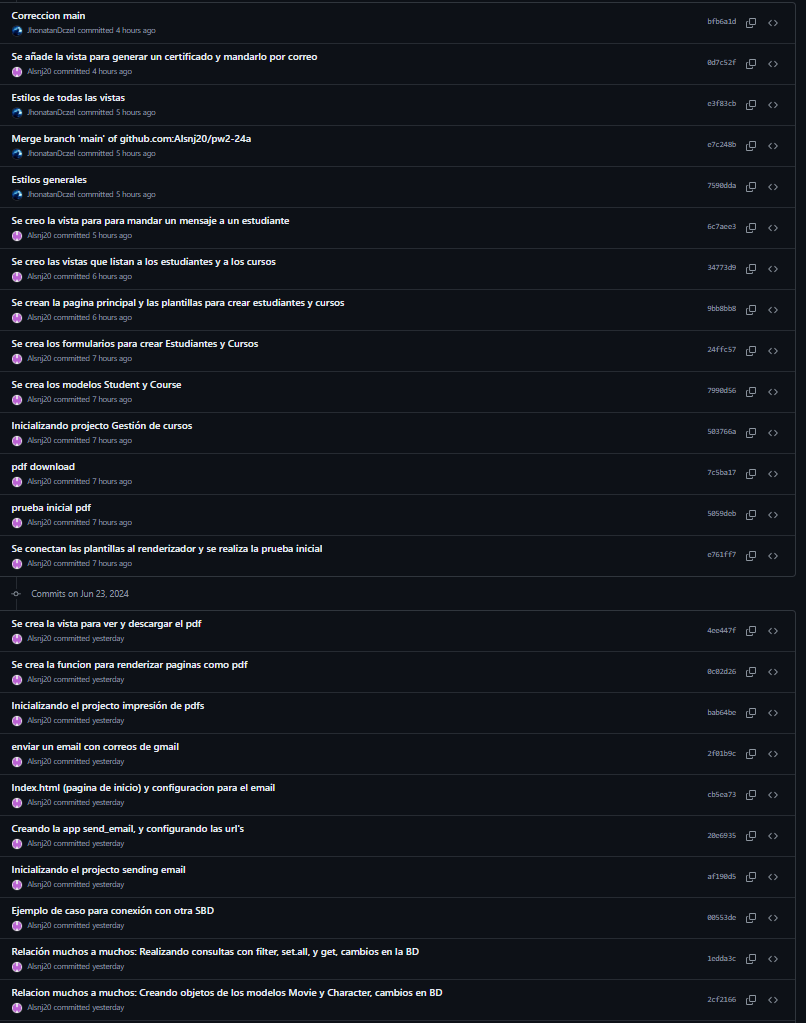
\includegraphics[width=0.9\textwidth,keepaspectratio]{img/commits.png}
	\caption{Lista de commits.}
\end{figure}
\pagebreak
\section{Equipos y materiales utilizados}
\begin{itemize}
	%%%%%%%%%%%%%%%%%%%%%%%%%%%%%%%%%%%%%%%%%%%%%%%%%%%%%%%%%%%%%%%%%%%%%%
	\item Cuenta en GitHub con el correo institucional.
	\item Sistema Operativo Microsoft Windows 10
	\item Visual Studio Code
	\item Git
	\item Windows PowerShell
	\item Python
	\item Navegador Mozilla Firefox
	      %%%%%%%%%%%%%%%%%%%%%%%%%%%%%%%%%%%%%%%%%%%%%%%%%%%%%%%%%%%%%%%%%%%%%%
\end{itemize}
\pagebreak

\section{Ejercicio 1: Relación: Uno a Muchos y Muchos a Muchos}
\subsection{Código}
\begin{block}
	\inputminted{python}{../relations_examples/example/models.py}
	\caption{Archivo models.py}
\end{block}
\subsection{Ejecución}

\subsubsection{Relación de uno a muchos}
Se muesta las operaciones realizar con los modelos Language y Framework.
\begin{figure}[H]
	\centering
	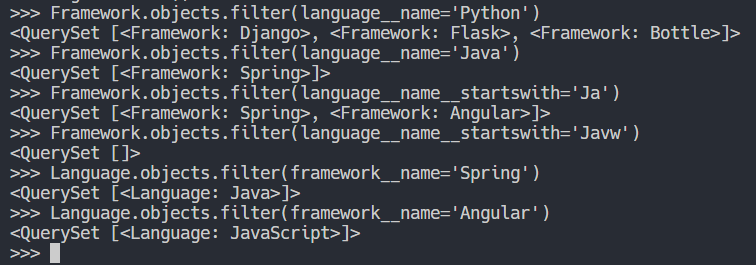
\includegraphics[width=0.9\textwidth,keepaspectratio]{img/r1operaciones.png}
	\caption{Resultado de la relación de uno a muchos.}
\end{figure}
\subsubsection{Relación de muchos a muchos}
Se muesta las operaciones realizar con los modelos Movie y Character.
\begin{figure}[H]
	\centering
	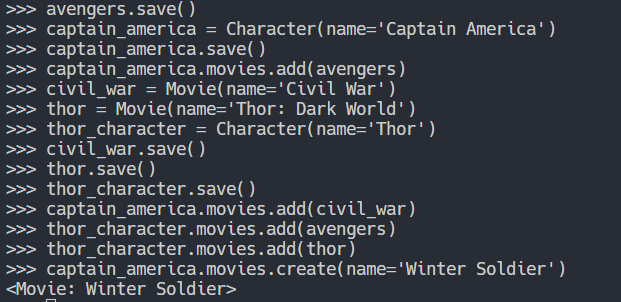
\includegraphics[width=0.9\textwidth,keepaspectratio]{img/r2operations.png}
	\caption{Resultado de la relación de muchos a muchos.}
\end{figure}

\subsection{Base de Datos}

\subsubsection{Relación de uno a muchos}
Se muesta la BD de los modelos Language y Framework.
\begin{figure}[H]
	\centering
	\begin{minipage}{0.4\textwidth}
		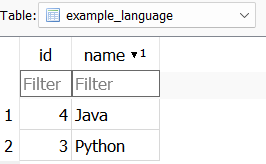
\includegraphics[width=\linewidth, height=5cm, keepaspectratio]{img/r1tabla1.png}
		\caption{Tabla Language.}
	\end{minipage}
	\hspace{0.5cm} % Espacio horizontal entre las dos imágenes
	\begin{minipage}{0.4\textwidth}
		\centering
		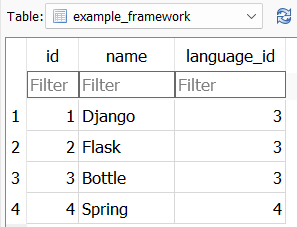
\includegraphics[width=\linewidth, height=5cm, keepaspectratio]{img/r1tabla2.png}
		\caption{Tabla Framework.}
	\end{minipage}
\end{figure}
\subsubsection{Relación de muchos a muchos}
Se muesta la BD de los modelos Movie y Character.
\begin{figure}[H]
	\centering
	\begin{minipage}{0.3\textwidth}
		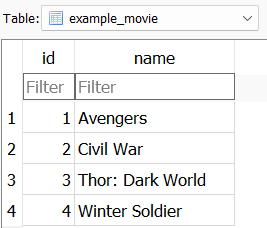
\includegraphics[width=\linewidth, height=5cm, keepaspectratio]{img/r2tabla1.png}
		\caption{Tabla Language.}
	\end{minipage}
	\hspace{0.5cm} % Espacio horizontal entre las dos imágenes
	\begin{minipage}{0.3\textwidth}
		\centering
		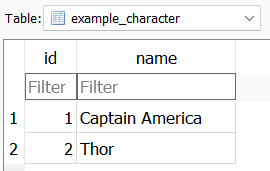
\includegraphics[width=\linewidth, height=5cm, keepaspectratio]{img/r2tabla2.png}
		\caption{Tabla Framework.}
	\end{minipage}
	\begin{minipage}{0.3\textwidth}
		\centering
		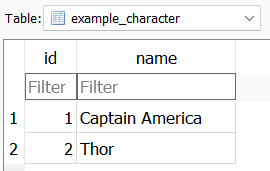
\includegraphics[width=\linewidth, height=5cm, keepaspectratio]{img/r2tabla2.png}
		\caption{Tabla Framework.}
	\end{minipage}
\end{figure}

\section{Ejercicio 2: Envio de correos electrónicos}
\subsection{Código}
Se muestra el archivo view.py para el envio del correo.
\begin{block}
	\inputminted{python}{../email_example/send_email/views.py}
	\caption{Archivo views.py}
\end{block}
\subsection{Prueba}

\begin{figure}[H]
	\centering
	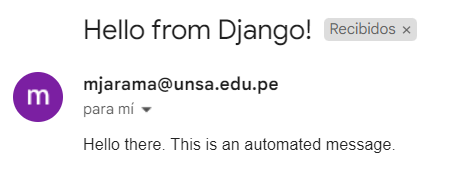
\includegraphics[width=0.6\textwidth,keepaspectratio]{img/send_email.png}
	\caption{Prueba del envio de email.}
\end{figure}

\section{Ejercicio 3: Impresión de PDFs}
\subsection{Código}
Para este ejercicio instalar la dependencia xhtml2pdf.
\begin{lstlisting}
	py -m pip install xhtml2pdf pip --upgrade
\end{lstlisting}
\begin{itemize}
	\item \textbf{renderers.py:} Contiene la función \texttt{render\_to\_pdf} que utiliza \texttt{pisa} para convertir una plantilla HTML y un diccionario de contexto en un documento PDF. Devuelve una respuesta HTTP con el PDF generado.
	      \begin{block}
		      \inputminted{python}{../print_pdfs/app/renderers.py}
		      \caption{Archivo renderers.py}
	      \end{block}
	\item \textbf{views.py:} Contiene la vista que renderiza la plantilla \texttt{invoice.html} y la convierte en un PDF.
	      \begin{block}
		      \inputminted{python}{../print_pdfs/app/views.py}
		      \caption{Archivo views.py}
	      \end{block}
	\item \textbf{invoice.html:} Contiene la plantilla HTML que se convertirá en un PDF.
	      \begin{block}
		      \inputminted{html}{../print_pdfs/app/templates/pdf/invoice.html}
		      \caption{Archivo invoice.html}
	      \end{block}
\end{itemize}

\subsection{Prueba}
\begin{figure}[H]
	\centering
	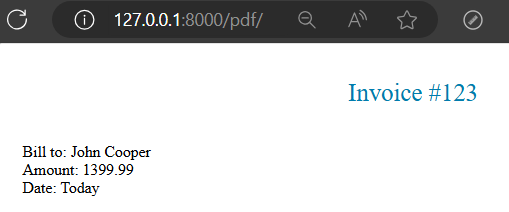
\includegraphics[width=0.6\textwidth,keepaspectratio]{img/print_pdf.png}
	\caption{Prueba de la impresión de PDFs.}
\end{figure}


\section{Ejercicio Propuesto: Sistema de Gestión de Cursos}
Se propone un sistema de gestión de cursos que permita a los estudiantes registrarse, registrar cursos junto con sus estudiantes, enviar mensajes por correo electrónico a los estudiantes y generar certificados en formato PDF para los estudiantes.
\subsection{Código}
\subsubsection{Modelos}
Define dos modelos de Django: \texttt{Student} y \texttt{Course}.
\begin{itemize}
	\item \texttt{Student} tiene campos \texttt{name} y \texttt{email}.
	\item \texttt{Course} tiene campos \texttt{name}, \texttt{teacher}, y una relación many-to-many con \texttt{Student}.
\end{itemize}
\begin{block}
	\inputminted{python}{../Course_Management_System/systemM/models.py}
	\caption{Archivo models.py}
\end{block}

\subsubsection{Formularios}
\begin{itemize}
	\item \texttt{StudentForm}: Formulario para registrar a un estudiante, basado en el modelo \texttt{Student} con campos \texttt{name} y \texttt{email}.
	\item \texttt{CourseForm}: Formulario para registrar un curso, basado en el modelo \texttt{Course} con campos \texttt{name}, \texttt{teacher} y \texttt{students} (usando \texttt{CheckboxSelectMultiple} para seleccionar varios estudiantes).
	\item \texttt{MessageForm}: Formulario para mandar un email a un estudiante \texttt{student} (\texttt{ModelChoiceField}), \texttt{course} (\texttt{ModelChoiceField}) y \texttt{message} (\texttt{CharField}).
	\item \texttt{CertifiedForm}: Formulario que debemos llenar para generar un certificado \texttt{student} (\texttt{ModelChoiceField}), \texttt{course} (\texttt{ModelChoiceField}) y \texttt{message} (\texttt{CharField}).
\end{itemize}
\begin{block}
	\inputminted{python}{../Course_Management_System/systemM/forms.py}
	\caption{Archivo forms.py}
\end{block}

\subsubsection{Vistas}
\begin{itemize}
	\item \texttt{index(request)}: Renderiza la página principal.
	\item \texttt{register\_student(request)}: Permite registrar nuevos estudiantes mediante un formulario.
	\item \texttt{register\_course(request)}: Permite registrar nuevos cursos mediante un formulario.
	\item \texttt{list\_students(request)}: Muestra todos los estudiantes registrados.
	\item \texttt{list\_courses(request)}: Muestra todos los cursos registrados.
	\item \texttt{send\_message(request)}: Envía un mensaje a un estudiante específico de un curso.
	\item \texttt{generate\_certified(request)}: Genera un certificado en formato PDF para un estudiante de un curso específico, lo adjunta a un correo electrónico y lo envía al estudiante.
\end{itemize}
\begin{block}
	\inputminted{python}{../Course_Management_System/systemM/views.py}
	\caption{Archivo views.py}
\end{block}

\subsection{Archivos Proyecto}
\subsubsection{Urls}
\begin{itemize}
	\item \texttt{index}: Página principal.
	\item \texttt{register\_student}: Para registrar estudiantes.
	\item \texttt{register\_course}: Para registrar cursos.
	\item \texttt{list\_students}: Para listar todos los estudiantes.
	\item \texttt{list\_courses}: Para listar todos los cursos.
	\item \texttt{send\_message}: Para enviar mensajes a estudiantes de cursos específicos.
	\item \texttt{generate\_certified}: Para generar certificados en formato PDF y enviarlos por correo electrónico.
\end{itemize}
\begin{block}
	\inputminted{python}{../Course_Management_System/systemM/urls.py}
	\caption{Archivo urls.py}
\end{block}
\subsubsection{Settings}
\begin{itemize}
	\item \texttt{INSTALLED\_APPS}: Se agregan la app \texttt{systemM}.
	\item \texttt{EMAIL\_HOST}, \texttt{EMAIL\_PORT}, \texttt{EMAIL\_HOST\_USER}, \texttt{EMAIL\_HOST\_PASSWORD}: Configuración para enviar correos electrónicos.
	\item \texttt{STATICFILES\_DIRS}: Se agrega la carpeta \texttt{static} para almacenar archivos estáticos.
	\item \texttt{EMAIL\_USE\_TLS}: Habilita el uso de TLS.
	\item \texttt{EMAIL\_USE\_SSL}: Habilita el uso de SSL.
	\item \texttt{EMAIL\_BACKEND}: Configuración para enviar correos. electrónicos.
\end{itemize}
\begin{block}
	\inputminted{python}{../Course_Management_System/system/settings.py}
	\caption{Archivo settings.py}
\end{block}

\subsection{Archivos Estaticos}
\subsubsection{HTML}
Estas plantillas HTML definen la interfaz de usuario para diversas funcionalidades:
\begin{itemize}
	\item \textbf{nav.html}: Plantilla base que define la estructura de navegación común a todas las páginas.
	      \begin{block}
		      \inputminted{html}{../Course_Management_System/systemM/templates/nav.html}
		      \caption{Archivo nav.html}
	      \end{block}

	\item \textbf{index.html}: Plantilla para la página principal del sistema.
	      \begin{block}
		      \inputminted{html}{../Course_Management_System/systemM/templates/index.html}
		      \caption{Archivo index.html}
	      \end{block}

	\item \textbf{register\_student.html}: Plantilla para registrar un nuevo estudiante.
	      \begin{block}
		      \inputminted{html}{../Course_Management_System/systemM/templates/register_student.html}
		      \caption{Archivo register\_student.html}
	      \end{block}

	\item \textbf{register\_course.html}: Plantilla para registrar un nuevo curso.
	      \begin{block}
		      \inputminted{html}{../Course_Management_System/systemM/templates/register_course.html}
		      \caption{Archivo register\_course.html}
	      \end{block}

	\item \textbf{list\_courses.html}: Plantilla para mostrar la lista de cursos registrados.
	      \begin{block}
		      \inputminted{html}{../Course_Management_System/systemM/templates/list_courses.html}
		      \caption{Archivo list\_courses.html}
	      \end{block}

	\item \textbf{list\_students.html}: Plantilla para mostrar la lista de estudiantes registrados.
	      \begin{block}
		      \inputminted{html}{../Course_Management_System/systemM/templates/list_students.html}
		      \caption{Archivo list\_students.html}
	      \end{block}

	\item \textbf{send\_message.html}: Plantilla para enviar un mensaje a los estudiantes.
	      \begin{block}
		      \inputminted{html}{../Course_Management_System/systemM/templates/send_message.html}
		      \caption{Archivo send\_message.html}
	      \end{block}

	\item \textbf{generate\_certified.html}: Plantilla que muestra el formulario para generar certificados.
	      \begin{block}
		      \inputminted{html}{../Course_Management_System/systemM/templates/generate_certified.html}
		      \caption{Archivo generate\_certified.html}
	      \end{block}
	\item \textbf{certified.html}: Plantilla que muestra el certificado generado.
	      \begin{block}
		      \inputminted{html}{../Course_Management_System/systemM/templates/certified.html}
		      \caption{Archivo certified.html}
	      \end{block}
\end{itemize}

\subsubsection{CSS}
\begin{itemize}
	\item \textbf{nav.css}: Estilo para la barra de navegación.
	      \begin{block}
		      \inputminted{CSS}{../Course_Management_System/systemM/templates/css/nav.css}
		      \caption{Archivo nav.css}
	      \end{block}

	\item \textbf{form-page.css}: Estilo para el formulario de registro de estudiantes y cursos.
	      \begin{block}
		      \inputminted{CSS}{../Course_Management_System/systemM/templates/css/form-page.css}
		      \caption{Archivo form-page.css}
	      \end{block}

	\item \textbf{lists.css}: Estilo para las listas de estudiantes y cursos.
	      \begin{block}
		      \inputminted{CSS}{../Course_Management_System/systemM/templates/css/lists.css}
		      \caption{Archivo lists.css}
	      \end{block}
\end{itemize}

\subsection{Prueba}
\section{Registro de Estudiantes}
\begin{figure}[H]
	\centering
	\begin{minipage}{0.6\textwidth}
		\centering
		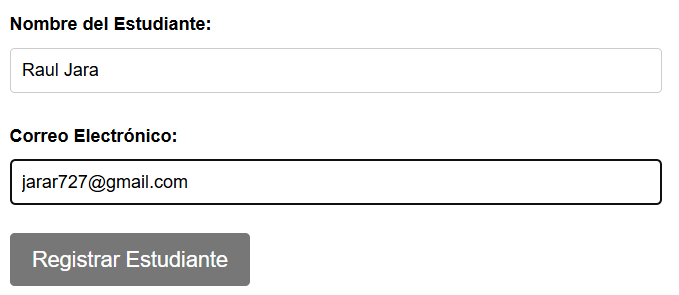
\includegraphics[width=\linewidth,keepaspectratio]{img/registerStudent.png}
		\caption{Registro de estudiantes.}
	\end{minipage}\hfill
	\begin{minipage}{0.4\textwidth}
		\centering
		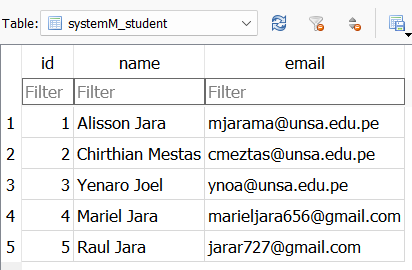
\includegraphics[width=\linewidth,keepaspectratio]{img/registerSBD.png}
		\caption{Registro de estudiantes en la base de datos.}
	\end{minipage}
\end{figure}

\section{Registro de Cursos}
\begin{figure}[H]
	\centering
	\begin{minipage}{0.3\textwidth}
		\centering
		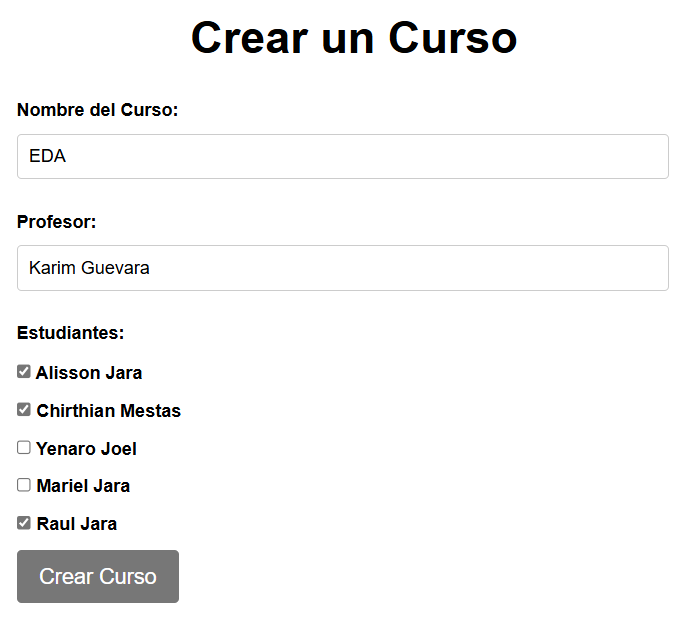
\includegraphics[width=\linewidth,keepaspectratio]{img/registerCourse.png}
		\caption{Registro de cursos.}
	\end{minipage}\hfill
	\begin{minipage}{0.3\textwidth}
		\centering
		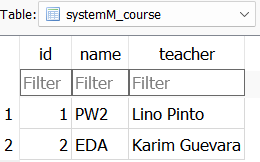
\includegraphics[width=\linewidth,keepaspectratio]{img/registerCBD.png}
		\caption{Registro de cursos en la base de datos.}
	\end{minipage}
	\begin{minipage}{0.3\textwidth}
		\centering
		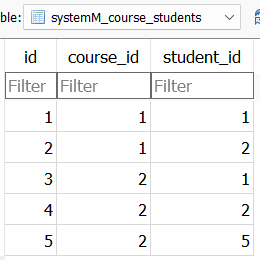
\includegraphics[width=\linewidth,keepaspectratio]{img/relation.png}
		\caption{Relación entre estudiantes y cursos.}
	\end{minipage}
\end{figure}

\section{Lista de Estudiantes}
\begin{figure}[H]
	\centering
	\begin{minipage}{0.6\textwidth}
		\centering
		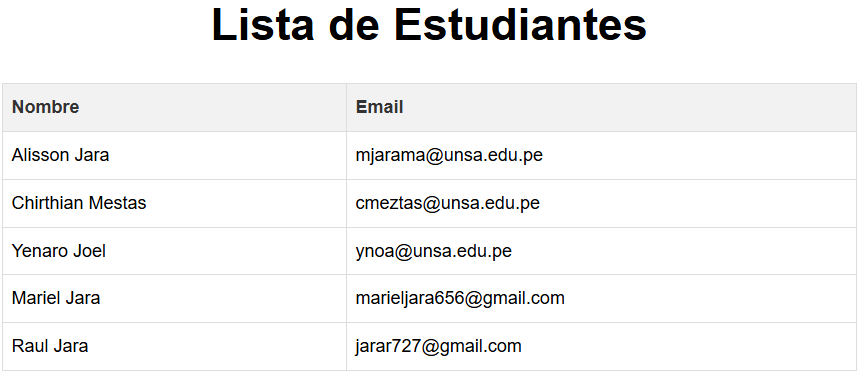
\includegraphics[width=\linewidth,keepaspectratio]{img/listStudents.png}
		\caption{Lista de estudiantes.}
	\end{minipage}
\end{figure}

\section{Lista de Cursos}
\begin{figure}[H]
	\centering
	\begin{minipage}{0.6\textwidth}
		\centering
		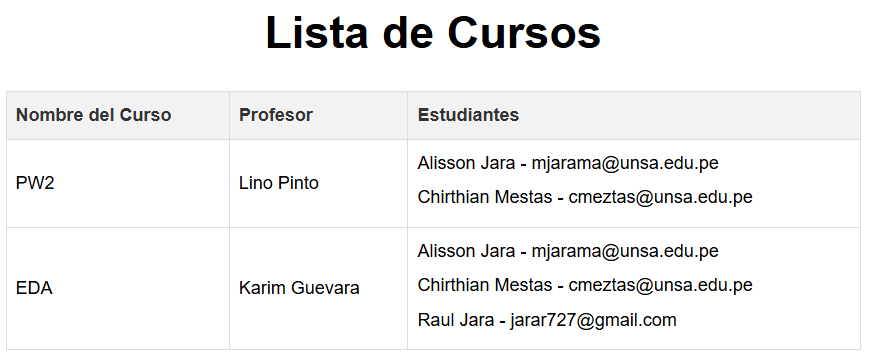
\includegraphics[width=\linewidth,keepaspectratio]{img/listCourses.png}
		\caption{Lista de cursos.}
	\end{minipage}
\end{figure}

\section{Envio de Mensajes}
\begin{figure}[H]
	\centering
	\begin{minipage}{0.6\textwidth}
		\centering
		
\includegraphics[width=\linewidth,keepaspectratio]{img/sendMessage.png}
		\caption{Envio de mensajes.}
	\end{minipage}
\end{figure}

\section{Generación de Certificados}
\begin{figure}[H]
	\centering
	\begin{minipage}{0.6\textwidth}
		\centering
		
\includegraphics[width=\linewidth,keepaspectratio]{img/certificado.png}
		\caption{Generación de certificados.}
	\end{minipage}
\end{figure}
\section{URL del repositorio en GitHub}
\begin{itemize}
	\item \url{https://github.com/Alsnj20/pw2-24a/tree/main/lab08}
\end{itemize}
\pagebreak
\section{Estructura de laboratorio \itemPracticeNumber}
\begin{itemize}
	\item El contenido que se entrega en este laboratorio es el siguiente:
\end{itemize}
\begin{lstlisting}{language=bash}
lab08/
	|--Course_Management_System/
		|--systemM/
			|--migrations/
			|--templates/
				|--css/
					|--form-page.css
					|--lists.css
					|--nav.css
				|--pdf/
					|--certified.html
					|--generate_certified.html
					|--index.html
					|--invoice.html
					|--list_courses.html
					|--list_students.html
					|--nav.html
					|--register_course.html
					|--register_student.html
					|--send_message.html
			|--__init__.py
			|--admin.py
			|--apps.py
			|--forms.py
			|--models.py
			|--renderers.py
			|--tests.py
			|--urls.py
			|--views.py
		|--system/
	|--relations_examples/
	|--email_example/
	|--print_pdfs/
|--Latex/
		|--linopinto_pw2_24a_lab08.tex
		|--linopinto_pw2_24a_lab08.pdf
		|--img/
			 |--commits.png
			 |--r1operaciones.png
			 |--r2operations.png
			 |--r1tabla1.png
			 |--r1tabla2.png
			 |--r2tabla1.png
			 |--r2tabla2.png
			 |--r2tabla3.png
			 |--send_email.png
			 |--print_pdf.png
			 |--registerStudent.png
			 |--registerSBD.png
			 |--registerCourse.png
			 |--registerCBD.png
			 |--relation.png
			 |--listStudents.png
			 |--listCourses.png
			 |--sendMessage.png
			 |--certificado.png
|--.gitignore
\end{lstlisting}
\section{Rúbrica}

\begin{table}[H]
	\centering
	\caption{Tabla: Rúbrica para contenido del Informe y evidencias}
	\begin{tabular}{|p{2cm}|p{6cm}|c|c|c|c|}
		\hline
		\multicolumn{2}{|c|}{\textbf{Contenido y demostración}} & \textbf{Puntos}                                                                                                                                                                                                                                                                  & \textbf{Checklist} & \textbf{Estudiante} & \textbf{Profesor}   \\ \hline
		1. GitHub                                               & Repositorio se pudo clonar y se evidencia la estructura adecuada para revisar los entregables. (Se descontará puntos por error o observación)                                                                                                                                    & 4                  & ×                   & 4                 & \\ \hline
		2. Commits                                              & Hay porciones de código fuente asociado a los commits planificados con explicaciones detalladas. (El profesor puede preguntar para refrendar calificación)                                                                                                                       & 4                  & ×                   & 4                 & \\ \hline
		3. Ejecución                                            & Se incluyen comandos para ejecuciones y pruebas del código fuente explicadas gradualmente que permitirían replicar el proyecto. (Se descontará puntos por cada omisión)                                                                                                          & 4                  & ×                   & 4                 & \\ \hline
		4. Pregunta                                             & Se responde con completitud a la pregunta formulada en la tarea. (El profesor puede preguntar para refrendar calificación)                                                                                                                                                       & 2                  & ×                   & 2                 & \\ \hline
		7.Ortografía                                            & El documento no muestra errores ortográficos. (Se descontará puntos por error encontrado)                                                                                                                                                                                        & 2                  & ×                   & 1                 & \\ \hline
		8. Madurez                                              & El Informe muestra de manera general una evolución de la madurez del código fuente con explicaciones puntuales pero precisas, agregando diagramas generados a partir del código fuente y refleja un acabado impecable. (El profesor puede preguntar para refrendar calificación) & 4                  & ×                   & 4                 & \\ \hline
		\multicolumn{2}{|c|}{\textbf{Total}}                    & 20                                                                                                                                                                                                                                                                               & Completo           & 19                  &                     \\ \hline
	\end{tabular}
\end{table}

\section{Referencias}
\begin{itemize}
	\item \url{https://github.com/}
	\item \url{https://git-scm.com/}
	\item \url{https://www.w3schools.com/python/}
\end{itemize}

\pagebreak
\bibliographystyle{apalike}
\bibliographystyle{IEEEtranN}
\bibliography{bibliography}

\end{document}